\chapter{OSLO-uitbreiding voor gegevens rond deelmobiliteit}
\label{chap:ontologie_voor_fietsdeeloperatoren}
\Glspl{mobop} publiceren hun gegevens in verschillende gegevensmodellen en -formaten waardoor die gegevenssets niet interoperabel zijn met andere gegevens van de Vlaamse overheid. Het OSLO mobiliteit: trips \& aanbod vocabularium zou een uitbreiding moeten krijgen zodat we gegevens rond deelmobiliteit in het OSLO-programma kunnen krijgen.
Om hiertoe te komen ligt de focus op het publiceren van gegevens rond Vlaamse fietsdeeloperatoren op een OSLO-conforme manier. Toch wordt het vocabularium op generieke wijze ontwikkeld zodat in een latere fase ook gegevens van andere deelmobiliteit-operatoren met datzelfde vocabularium kunnen worden gepubliceerd.
Net daarom wordt de GBFS-specificatie gekozen als vertrekpunt bij deze ontwikkeling.
GBFS biedt de nodige object-eigenschappen en structuur die nodig zijn in een model voor dergelijke gegevens.
Er wordt in de GBFS-specificatie abstract te werk gegaan door de mogelijkheid te bieden om gegevens met betrekking tot verschillende vervoermiddel-types aan een station te koppelen. 
Dit wordt aangepakt door een container van objecten als waarde van een eigenschap, zoals aantal items beschikbaar voor gebruik, te aanvaarden.
Bijlage F is een snipit uit een voorbeeld van een object dat stationsinformatie bevat. Het object-eigenschap ``vechicle\_types\_available'' is een term waarbij die abstracte implementatie werd toegepast.
Het zijn de termen, uit het gegevensmodel `station\_status' van de GBFS-specificatie, die worden hergebruikt om een uitbreiding voor OSLO te ontwikkelen. 

In de secties die volgen wordt beschreven hoe de uitbreiding op OSLO mobiliteit: trips \& aanbod, als voorstel om op te nemen in het vocabularium, tot stand zijn gekomen. De uitbreiding is niet volledig, maar generiek zodat er aan kan worden verder gebouwd indien het vocabularium wordt opgenomen in OSLO.
In tabel \ref{tab:oslo_prefixes} staan enkele OSLO-prefixes waarnaar zal worden verwezen in onderstaande secties. De technische informatie van iedere RDF-klasse waarnaar wordt gerefereerd kan worden teruggevonden door de URI te volgen gevormd door de prefix geconcateneerd met de RDF-term.

\begin{table}[]
\centering
\caption{gebruikte prefixes}
\label{tab:oslo_prefixes}
\begin{tabular}{ll}
ext:     & \url{https://stijnbrysbaert.github.io/OSLO-extension/vocabulary.ttl#} \\
dct   & \url{http://purl.org/dc/terms/} \\
mob   & \url{https://data.vlaanderen.be/ns/mobiliteit-trips-en-aanbod#} \\
net   & \url{https://data.vlaanderen.be/ns/netwerk#}         \\
tn    & \url{https://data.vlaanderen.be/ns/transportnetwerk#} \\
rdf   & \url{https://www.w3.org/1999/02/22-rdf-syntax-ns#} \\
weg   & \url{https://data.vlaanderen.be/ns/weg#}
\end{tabular}
\end{table}

\section{Station}
Allereerst is er nood aan een `Station'-klasse dat individuen van stations omschrijft. Een station in deze context is een object in het mobiliteitslandschap waar vervoermiddelen kunnen geparkeerd en gebruikt worden. Afgeleid uit het GBFS station-status gegevensmodel\footnote{\url{https://github.com/NABSA/gbfs/blob/master/gbfs.md\#station_statusjson}} kan een station de real-time beschikbaarheid van voertuigen weergeven. In de GBFS-specificatie wordt de capaciteit en beschikbaarheid van voertuigen gemodelleerd zodat het mogelijk is die eigenschappen bij te houden voor meerdere verschillende soorten vervoermiddelen (zie bijlage F): (elektrische)fiets, auto, step, ... Op die manier kan de gegevensset van een station worden aangevuld wanneer er een nieuw type voertuig wordt in ondergebracht.

\textit{tn:Transportpunt} kan als superklasse worden gebruikt voor deze nieuwe klasse om een connectie te voorzien naar OSLO. Deze superklasse is zelf een subklasse van \textit{tn:Transportobject} en \textit{tn:Netwerkelement} en kan worden gelinkt aan een geografisch punt met het \textit{tn:geometrie} predicaat.

\begin{table}[h]
\centering
\begin{tabular}{|l|l|}
\hline
\textbf{type}     & \textbf{klasse}                                                                                \\ \hline
URI               & {\color[HTML]{000000} ext:Station} \\ \hline
Specialisatie van & \begin{tabular}[c]{@{}l@{}}\url{https://data.vlaanderen.be/ns/transportnetwerk#Transportpunt}\\ \end{tabular} \\ \hline
Definitie         & Station waar voertuigen kunnen worden geplaatst en gebruikt.                                   \\ \hline
\end{tabular}
\end{table}

\section{VoertuigenBeschikbaar}
Het idee uit de GBFS-specificatie om gegevens van verschillende types vervoermiddelen in eenzelfde station bij te houden, nemen we over naar deze OSLO-uitbreiding. De klasse waarin het aantal beschikbare voertuigen, bijvoorbeeld deelfietsen, wordt gemodelleerd, moet generiek zijn. De VoertuigenBeschikbaar-klasse zal voor een specifiek vervoermiddel bijhouden hoeveel items er op dat moment beschikbaar zijn om te gebruiken. In dit domein kunnen twee eigenschappen worden aanvaard: \textit{ext:aantal} en \textit{dct:type}. Van deze klasse kunnen er meerdere instanties gelinkt worden aan de station instantie.

\begin{table}[h]
\centering
\begin{tabular}{|l|l|}
\hline
\textbf{type}     & \textbf{klasse}                                                                                \\ \hline
URI               & {\color[HTML]{000000} ext:VoertuigenBeschikbaar} \\ \hline
Definitie         & Het aantal voertuigen van een bepaalt type dat beschikbaar is.                                   \\ \hline
\end{tabular}
\end{table}

\subsection{aantal}
De \textit{ext:aantal} eigenschap duidt het aantal voertuigen van een bepaald vervoermiddel aan.

\begin{table}[h]
\centering
\begin{tabular}{|l|l|}
\hline
\textbf{type}     & \textbf{eigenschap}                                                                                \\ \hline
URI               & {\color[HTML]{000000} ext:aantal} \\ \hline
Definitie         & Aantal items van een instantie  \\ \hline
Domein & \begin{tabular}[c]{@{}l@{}}ext:VoertuigenBeschikbaar\\ext:VoertuigenDocks\end{tabular} \\ \hline
Bereik & \url{http://www.w3.org/2001/XMLSchema#integer} \\ \hline
\end{tabular}
\end{table}

\subsection{type}
De \textit{dct:type} eigenschap verwacht volgens het applicatieprofiel van OSLO mobiliteit: trips \& aanbod een instantie van het rdf type Resourcetype. Resourcetype werd echter nog niet gedefinieerd in het applicatieprofiel. Het omschrijven van deze klasse valt buiten de scope van deze scriptie. 

% In het wegen-vocabularium\footnote{\url{https://data.vlaanderen.be/ns/weg}} bestaat er een eigenschap weg:voertuigtype dat ook ideaal lijkt om het type voertuig aan te duiden. Deze eigenschap kan helaas enkel worden toegepast worden in het weg:Rijrichting domein. Er zal een weloverwogen beslissing moeten worden gemaakt over welke RDF term zal worden 

\section{DocksBeschikbaar}
De klasse `DocksBeschikbaar' krijgt dezelfde eigenschappen als de VoertuigenBeschikbaar-klasse: aantal en type. De klasse houdt het aantal \glspl{dock} dat beschikbaar is in een station voor een bepaald vervoermiddel bij.

\section{Beschikbaarheid}
De beschikbaarheid-klasse gedefinieerd in OSLO mobiliteit: trips \& aanbod kan gelinkt worden aan een station en bevat instanties die betrekking hebben tot de mate waarin iets voorhanden is voor gebruik. Een station heeft exact één instantie van de beschikbaarheid-klasse en wordt met behulp van de \textit{mob:Transportobject.beschikbaarheid} eigenschap gelinkt. Gezien een station een subklasse is van \textit{mob:Transportpunt} en die klasse op zijn beurt weer een subklasse is van \textit{mob:Transportobject}, wordt de \textit{mob:Transportobject.beschikbaarheid} eigenschap binnen het juiste domein gebruikt.

Wat volgt zijn twee eigenschappen toepasbaar op de \textit{mob:Beschikbaarheid}-klasse waarmee gegevens rond de beschikbaarheid van voertuigen en docks in een station kunnen worden gelinkt.

\subsection{voertuigTypesBeschikbaar}
Deze eigenschap vormt de relatie tussen de beschikbaarheids-instantie van een station met het real-time aantal beschikbare voertuigen van een bepaalt type.

\begin{table}[h]
\centering
\begin{tabular}{|l|l|}
\hline
\textbf{type}     & \textbf{eigenschap} \\ \hline
URI               & ext:voertuigTypesBeschikbaar \\ \hline
Definitie         & Het aantal voertuigen van een bepaalt type dat beschikbaar is.                                   \\ \hline
Domein & mob:Beschikbaarheid \\ \hline
Bereik & ext:VoertuigenBeschikbaar \\ \hline
\end{tabular}
\end{table}

\subsection{voertuigDocksBeschikbaar}
Deze eigenschap vormt de relatie tussen de beschikbaarheids-instantie van een station met het real-time aantal beschikbare docks voor een bepaalt type voertuig. 

\begin{table}[h]
\centering
\begin{tabular}{|l|l|}
\hline
\textbf{type}     & \textbf{eigenschap} \\ \hline
URI               & ext:voertuigDocksBeschikbaar \\ \hline
Definitie         & Beschikbaarheid van het aantal plaatsen specifiek voor een bepaald type voertuig.  \\ \hline
Domein & mob:Beschikbaarheid \\ \hline
Bereik & ext:DocksBeschikbaar \\ \hline
\end{tabular}
\end{table}

\section{Voorbeeld}
Figuur~\ref{fig:rdf_gegevensset_voorbeeld} beeldt de graaf af die een mogelijke gegevensset, gepubliceerd volgens de OSLO-uitbreiding, visualiseert. Dankzij de klasses `VoertuigTypesBeschikbaar' en `DocksBeschikbaar' kunnen er onbeperkt aantal instanties gelinkt worden die per type voertuig informatie bevat.

\begin{figure}[h]
	\centering
	\begin{subfigure}{\textwidth}
		\centering
		\centerline{
			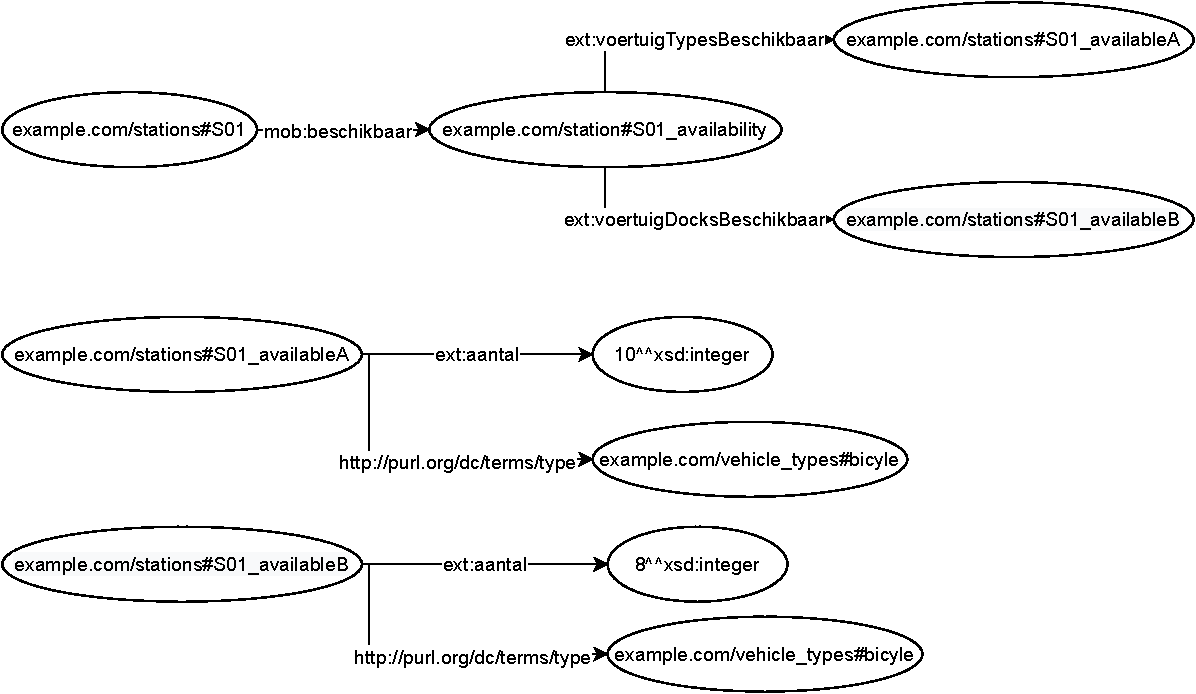
\includegraphics[width=\textwidth]{images/rdf_dataset.pdf}
		}
	\end{subfigure}
	\caption{Gegevensset gebruikmakend van RDF-model}
	\label{fig:rdf_gegevensset_voorbeeld}
\end{figure}